\documentclass[a4paper,12pt,twocolumn,landscape]{article}

\usepackage{superpack2015}
\usepackage{tkz-fct}

\usepackage[heightrounded]{geometry}	% heightrounded permet d'afficher les footers correctement
\geometry{hmargin=0.5cm,vmargin=1.5cm}

\setlength{\columnseprule}{0.5pt}		% Ligne séparatrice milieu document
\setlength{\columnsep}{50pt}			% Espace de chaque côté de la ligne
\setlength{\headsep}{15pt}
\addtolength{\textheight}{20pt}
%\setlength{\textwidth}{770pt}
%\setlength{\hoffset}{20pt}

\classichf
	% Nom du style
	{sujet}
	% Hauteur sous header
	% 14.5pt si une ligne (1 \baselineskip)
	% 29.0pt si deux lignes (2 \baselineskip)
	{14.5pt}
	% Head
	{}
	{\textbf{Exercices : Généralités sur les fonctions}}
	{}
	% Foot
	{}
	{}
	{}

%\usepackage{showframe}
%\usepackage{layout}

\begin{document}
\pagestyle{sujet}	%\thispagestyle{premierepage} pour isoler des styles de pages


\exercice Reprenons la fonction $h$ évoquée dans l'activité
\vspace*{-1em}
\begin{center}
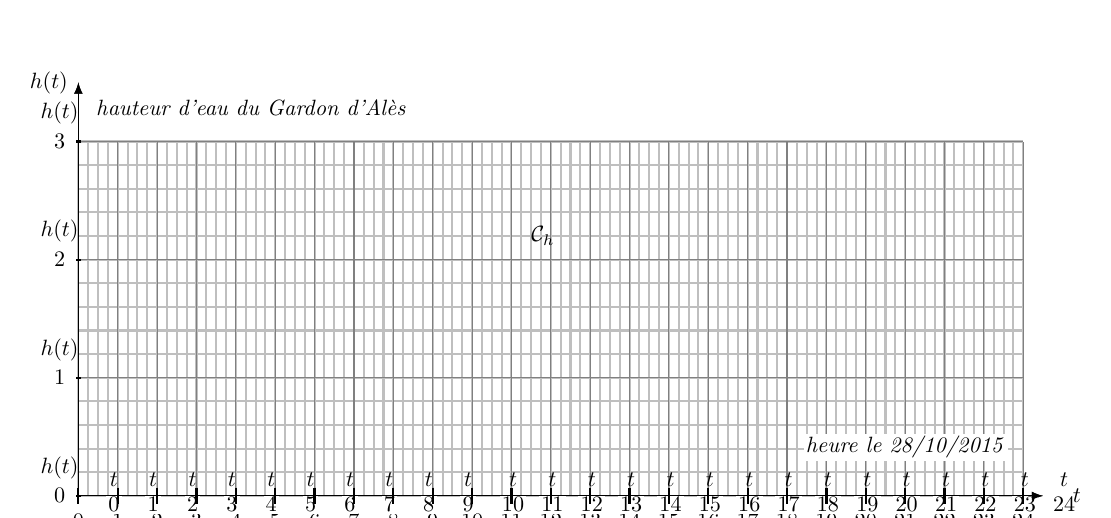
\begin{tikzpicture}[scale=0.5,yscale=3,every node/.style={scale=0.8}]
\tkzInit[xmax=24,xstep=1,ymax=3,ystep=1]
\tkzGrid[sub,
		subxstep=0.25,
		color=gray]
\tkzLabelX
\tkzDrawX[label={\textit{heure le 28/10/2015}},above left=18pt,fill=white]
\tkzLabelY
\tkzDrawY[label={\textit{hauteur d'eau du Gardon d'Al\`es}},below right=8pt]
\draw plot[smooth] file {ales.table.suite};
\tkzAxeX[label=$t$,right=10pt]
\tkzAxeY[label=$h(t)$]
\tkzText(11.8,2.2){$\mathcal{C}_{h}$}
\end{tikzpicture}
\end{center}

\begin{enumerate}
	\item Résoudre graphiquement $h(t) > 2$.
	\item Déterminer graphiquement les antécédents de $2$ par $h$.
	\item Déterminer graphiquement $h(22)$.
	\item Déterminer graphiquement le maximum de la fonction $h$ et la valeur de $t$ pour laquelle on l'obtient.
	\item Déterminer graphiquement les valeurs de~$t$ pour lesquelles la fonction~$h$ est croissante et celles où la fonction~$h$ est décroissante.
	\item Exprimer les réponses de la question précédente sous forme d'intervalles de valeurs de $t$.
	\item Pour chacune des questions précédentes, exprimer en langage courant ce qui est demandé.
	\item Répondre maintenant aux questions de 1. à \addtocounter{enumi}{-2}\theenumi \addtocounter{enumi}{2}.
\end{enumerate}	
\addtocounter{exercice}{1}
\paragraph*{Exercices \theexercice~à\addtocounter{exercice}{4}~\theexercice}~\\
\addtocounter{exercice}{-5}

\noindent Le carré $ABCD$ a un côté de longueur 8 cm.\\
$M$ est un point du segment $[AB]$.\\
On dessine dans le carré $ABCD$ :
\begin{itemize}
	\item Un carré de côté $[AM]$
	\item Un triangle isocèle de base $[MB]$ et dont la hauteur a même mesure que le côté $[AM]$ du carré.
\end{itemize}
Trois dessins sont proposés pour trois positions différentes du point $M$.\\


\def\echelle{0.8}
\def\couleur{red!50}
\begin{tikzpicture}[scale=\echelle,every node/.style={scale=\echelle}]
	\coordinate (A) at (0,0);
	\coordinate (B) at (4,0);
	\coordinate (C) at (4,4);
	\coordinate (D) at (0,4);
	\coordinate (M) at (1,0);
	\draw (A)--(B)--(C)--(D)--cycle;
	\draw[fill=\couleur] (A) rectangle (1,1);
	\draw[fill=\couleur] (M) -- (2.5,1) -- (B) -- cycle;
	\draw[dashed] (1,1) -- (4,1);
	\draw (M) node[below] {$M$};
	\draw (A) node[below left] {$A$};
	\draw (B) node[below right] {$B$};
	\draw (C) node[above right] {$C$};
	\draw (D) node[above left] {$D$};
\end{tikzpicture}
\begin{tikzpicture}[scale=\echelle,every node/.style={scale=\echelle}]
	\coordinate (A) at (0,0);
	\coordinate (B) at (4,0);
	\coordinate (C) at (4,4);
	\coordinate (D) at (0,4);
	\coordinate (M) at (2,0);
	\draw (A)--(B)--(C)--(D)--cycle;
	\draw[fill=\couleur] (A) rectangle (2,2);
	\draw[fill=\couleur] (M) -- (3,2) -- (B) -- cycle;
	\draw[dashed] (2,2) -- (4,2);
	\draw (M) node[below] {$M$};
	\draw (A) node[below left] {$A$};
	\draw (B) node[below right] {$B$};
	\draw (C) node[above right] {$C$};
	\draw (D) node[above left] {$D$};
\end{tikzpicture}
\begin{tikzpicture}[scale=\echelle,every node/.style={scale=\echelle}]
	\coordinate (A) at (0,0);
	\coordinate (B) at (4,0);
	\coordinate (C) at (4,4);
	\coordinate (D) at (0,4);
	\coordinate (M) at (3,0);
	\draw (A)--(B)--(C)--(D)--cycle;
	\draw[fill=\couleur] (A) rectangle (3,3);
	\draw[fill=\couleur] (M) -- (3.5,3) -- (B) -- cycle;
	\draw[dashed] (3,3) -- (4,3);
	\draw (M) node[below] {$M$};
	\draw (A) node[below left] {$A$};
	\draw (B) node[below right] {$B$};
	\draw (C) node[above right] {$C$};
	\draw (D) node[above left] {$D$};
\end{tikzpicture}

\exercice Dans quelle situation a-t-on l'aire du triangle la plus grande ?
\exercice Dans quelle situation l'aire du carré est égale à celle du triangle ?
\exercice Dans quelle situation l'aire du motif est elle égale à la moitié de celle de ABCD ?
\exercice Dans quelle situation a-t-on l'aire du triangle supérieure à la moitié de celle du carré ?
\exercice Comment évolue l'aire du motif en fonction de AM ? en fonction de MB ?

\exercice ~\\

Soient $f$ et $g$ deux fonctions affines~: $f(x)=x-2$ et $g(x)=-2x+1$
\begin{enumerate}
	\item Résoudre $x - 2 = -2x + 1$.
	\item Tracer $f$ et $g$ dans un repère d'unité 1 cm. $x \in \left[-1~;~2\right], y \in \left[-3~;~3\right]$
	\item Que signifie $f(x) = g(x)$ ?
	\item Que signifie $f(x) \geqslant g(x)$ ?
\end{enumerate}
\exercice~\\

\begin{minipage}{0.25\textwidth}
	\definecolor{xdxdff}{rgb}{0.49,0.49,1}
\definecolor{cqcqcq}{rgb}{0.75,0.75,0.75}
\begin{tikzpicture}[line cap=round,line join=round,>=triangle 45,x=1.0cm,y=1.0cm,scale=0.75,xscale=2.45,yscale=0.9,scale=1,every node/.style={scale=0.9}]
\draw [color=cqcqcq,dash pattern=on 2pt off 2pt, xstep=1cm,ystep=3.0cm] (-0.27,-4.53) grid (3.21,6.6);
\draw[->,color=black] (-0.27,0) -- (3.21,0);
\foreach \x in {,0.5,1,1.5,2,2.5,3}
\draw[shift={(\x,0)},color=black] (0pt,2pt) -- (0pt,-2pt) node[below] {\footnotesize $\x$};
\draw[->,color=black] (0,-4.53) -- (0,6.6);
\foreach \y in {-4,-3,-2,-1,1,2,3,4,5,6}
\draw[shift={(0,\y)},color=black] (2pt,0pt) -- (-2pt,0pt) node[left] {\footnotesize $\y$};
\draw[color=black] (0pt,-10pt) node[right] {\footnotesize $0$};
\clip(-0.27,-4.53) rectangle (3.21,6.6);
\draw[smooth,samples=100,domain=-0.27358351729212455:3.2128525876870215] plot(\x,{4*(\x)^2-12*(\x)+5});
\draw [domain=-0.27:3.21] plot(\x,{(--10-8*\x)/2});
\draw (0.67,3) node[anchor=north west] {$g$};
\draw (2.5,2.83) node[anchor=north west] {$f$};
\begin{scriptsize}
\fill [color=xdxdff] (2,-3) circle (1.5pt);
\draw[color=xdxdff] (2.15,-2.79) node {$B$};
\fill [color=xdxdff] (0,5) circle (1.5pt);
\draw[color=xdxdff] (0.09,5.24) node {$A$};
\end{scriptsize}\end{tikzpicture}
\end{minipage}
\hfill
\begin{minipage}{0.17\textwidth}
Résoudre
\begin{enumerate}
	\item $f(x) = 0$
	\item $f(x) \leqslant 0$\\
	\item $f(x) = 5$
	\item $f(x) \leqslant 5$\\
	\item $f(x) = g(x)$
	\item $f(x) \leqslant g(x)$\\
	\item $0 \leqslant f(x) \leqslant 5$
	\item $-3 \leqslant f(x) \leqslant 0$
\end{enumerate}
\end{minipage}
\exercice~\\[1em]
\noindent 
\begin{minipage}{0.22\textwidth}
	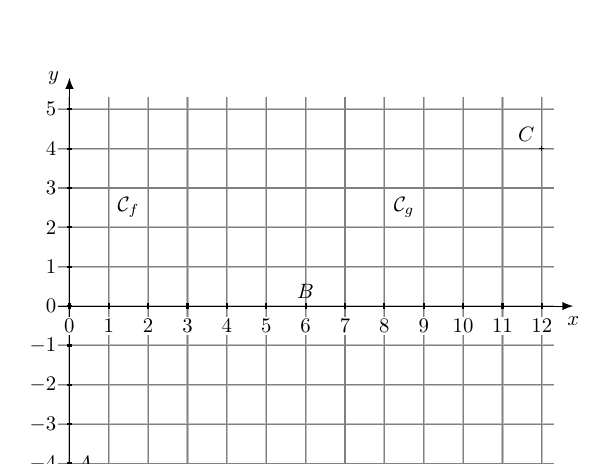
\begin{tikzpicture}[scale=0.5,xscale=1,every node/.style={scale=0.75}]
\tkzSetUpPoint[shape=cross]%,size=20pt,color=teal,fill=teal]
\tkzInit[xmin=-0.3,xmax=12.3, ymin=-4.3,ymax=5.3]
\tkzGrid[sub,subxstep=1,subystep=1]
\tkzAxeXY
\tkzFct[smooth,samples=20,domain = -0.3:12.3]{0.05833*(\x)**3-1.05*(\x)**2+4.86667*(\x)-4}
\tkzFct[samples=2,domain = -0.3:12.3]{(-48+8*\x)/12}
\tkzDefPointByFct[draw,ref=A](0)
\tkzLabelPoint[right](A){$A$}
\tkzCrossPoint{A}
\tkzDefPointByFct[draw,ref=B](6)
\tkzLabelPoint[above](B){$B$}
\tkzCrossPoint{B}
\tkzDefPointByFct[draw,ref=C](12)
\tkzLabelPoint[above left](C){$C$}
\tkzCrossPoint{C}
\tkzText(8.5,2.5){$\mathcal{C}_{g}$}
\tkzText(1.5,2.5){$\mathcal{C}_{f}$}
\end{tikzpicture}
\end{minipage}
\hfill
\begin{minipage}{0.23\textwidth}
\begin{enumerate}
	\item Dresser le \underline{tableau de variation} de~$f$ pour \mbox{$x \in [0~;~12]$}.\\
	\item Dresser le \underline{tableau de signes} de~$g$ pour \mbox{$x \in [0~;~12]$}.\\
	\item Entourer la bonne solution sur chaque ligne du tableau.
\end{enumerate}
\end{minipage}
\vspace*{2em}
\begin{center}
\begin{tabular}{|c|c|}
\hline 
\rule[-1ex]{0pt}{2.5ex} $f(x) \leqslant g(x)$ pour $x \in [0~;~6]$ & $f(x) \leqslant g(x)$ pour $x \in [6~;~12]$ \\ 
\hline 
\rule[-1ex]{0pt}{2.5ex} $f(x) \geqslant 0$ pour $x \in [1~;~6]$ & $f(x) \geqslant 0$ pour $x \in [6~;~11]$ \\ 
\hline 
\rule[-1ex]{0pt}{2.5ex} $f(x) \leqslant 0$ pour $x \in [6~;~11]$ & $f(x) \leqslant 0$ pour $x \in [0~;~1] \cup [6~;~11]$ \\ 
\hline 
\end{tabular} 
\end{center}
\exercice On considère le quadrilatère tournant vu à l'activité~1~:\\[1em] \noindent
$ABCD$ représente une feuille au format~$A4$ c'est-à-dire un rectangle de côtés $AB = 29,7cm$ et $BC = 21cm$.\\
On place $M$ sur $[AB]$.\\
On place ensuite $N$ sur $[BC]$, $P$ sur $[CD]$ et $Q$ sur $[DA]$ tels que~:\\ $AM = BN = CP = DQ$\\[1em]
On pose $x$ la longueur $AM$.\\[1em]
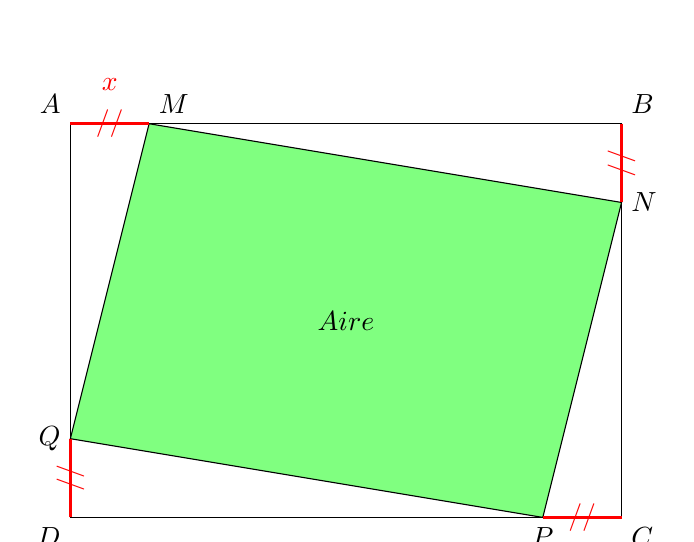
\begin{tikzpicture}[scale=1,every node/.style={scale=1}]
	\coordinate (A) at (0,0);
	\coordinate (B) at (7,0);
	\coordinate (C) at (7,-5);
	\coordinate (D) at (0,-5);
	\coordinate (M) at (1,0);
	\coordinate (N) at (7,-1);
	\coordinate (P) at (6,-5);
	\coordinate (Q) at (0,-4);
	\coordinate (S) at (7/2,-5/2);
	\draw (A) rectangle ++(7,-5);
	\draw (A)--(B)--(C)--(D)--cycle;
%	\draw [very thick,red] (A)--(M) node [midway,above] {$x$};
	\draw [black,fill=green!50] (M)--(N)--(P)--(Q)--cycle;
	\draw (A) node[above left] {$A$};
	\draw (B) node[above right] {$B$};
	\draw (C) node[below right] {$C$};
	\draw (D) node[below left] {$D$};
	\draw (M) node[above right] {$M$};
	\draw (N) node[right] {$N$};
	\draw (P) node[below] {$P$};
	\draw (Q) node[left] {$Q$};
	\draw (S) node {$Aire$};
%	\foreach \point in {A, B, C, D}
%		\draw (\point) node[above left] {$\point$};
	\draw [red,very thick] (A)--(M)node[midway,sloped]{$//$};
	\draw [red,very thick] (B)--(N)node[midway,sloped]{$//$};
	\draw [red,very thick] (C)--(P)node[midway,sloped]{$//$};
	\draw [red,very thick] (D)--(Q)node[midway,sloped]{$//$};
	\draw (0.5,0.5) node [red] {$x$};
\end{tikzpicture}
\\[1em]
\begin{enumerate}
	\item Montrez que l'aire verte peut s'écrire comme une fonction de $x$ dont on précisera le domaine de définition. On note cette fonction~$f$ et on a $f(x) = 2x^2 - 50,7x + 623,7$
\end{enumerate}
\newpage
\input{fonctions1-td-exercice104}
\newpage
\exercice~\\
Soit la fonction $f$ définie sur $\mathbb{R}$ par : $f(x) = 4x^2 + 24x + 35$ (\textbf{Expression~1})

On donne d’autres expressions possibles de la fonction $f$~:

\begin{enumerate}[~~~~]
	\vspace*{\stretch{1}}
	
	\item \textbf{Expression~2} $4(x + 3)^2 - 1$
	
	\vspace*{\stretch{1}}
	
	\item \textbf{Expression~3} $(2x + 5)(2x + 7)$
	
	\vspace*{\stretch{1}}
\end{enumerate}

\begin{enumerate}
	\item En développant les expressions 2 et 3, vérifier que toutes deux représentent bien la fonction $f$.
	\item Dans chaque situation proposée ci-dessous, en choisissant l’expression la plus appropriée, répondre à la question posée :
	\begin{enumerate}
		\item Déterminer l’image par $f$ de $-1$.
		\item Déterminer $f(-3)$.
		\item Déterminer les antécédents de $35$.
		\item Déterminer l’image de $\sqrt{2}$.
		\item Déterminer les antécédents de $-1$.
	\end{enumerate}
\end{enumerate}	 

\vspace*{\stretch{1}}

\exerciceprime~\\
Soit la fonction $g$ définie sur $\mathbb{R}$ par : $g(x) = 2x^2 + 7x - 4$ (\textbf{Expression~1})

On donne d’autres expressions possibles de la fonction $g$.
\begin{enumerate}
	\item Parmi les expressions suivantes indiquer en justifiant par un développement celles qui représentent aussi la fonction $g$.

	\vspace*{\stretch{1}}

	\textbf{Expression~2} $(2x - 1)(x + 4)$

	\vspace*{\stretch{1}}

	\textbf{Expression~3} $(2x - 1)(x + 1) + 3(2x - 1)$

	\vspace*{\stretch{1}}

	\textbf{Expression~4} $2(x + 3)^2 - 3x - 22$
	
	\vspace*{\stretch{1}}	
	
	\item Dans chaque situation proposée ci-dessous, en choisissant l’expression la plus appropriée qui est effectivement une expression de $g(x)$, répondre à la question posée :
	\begin{enumerate}
		\item Déterminer l’image par $g$ de $-1$.
		\item Déterminer $g(-4)$.
		\item Déterminer les antécédents de $0$ pour la fonction $g$.
		\item Déterminer l’image de $\sqrt{2}$ par la fonction $g$.
	\end{enumerate}
\end{enumerate}

\vspace*{\stretch{1}}


\end{document}


%
%%\exercicebareme{4}
%\exercicebareme{6}
%\exercicebareme{10}
%\exerciceunpoint
%\exercicebonus
%\FIN
%\BONNESVACANCES
%\BONCOURAGE
%\hrulefill